\scanpage{20}nier (ou, ce qui revient au même, $c$) est bien déterminée. Les unipotents qui définissent ladite filtration, en termes d'un $i$ qui la définit, sont
% Typed interlinear insertion; the pen line curls up at its right end and down to the left of de.
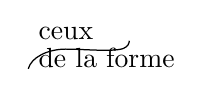
\begin{tikzpicture}[baseline=(base.base),x=1em,y=1ex]
  \node[anchor=base west,inner sep=0pt] (base) at (0,0) {de la forme};
  \node[anchor=base west,inner sep=0pt] at (0,2.35) {\inserted{ceux}};
  \draw[line width=.45pt] (-.35,-.10) .. controls (-.25,.85) and (.35,1.55) .. (1.00,1.55)
    .. controls (1.70,1.55) and (2.70,1.30) .. (3.08,1.60)
    .. controls (3.25,1.75) and (3.30,2.05) .. (3.30,2.25);
\end{tikzpicture}
$\exp(e)$, où $e$ parcourt $\handwritten{\unsure{\mathfrak{g}|\mathscr{G}}}(2)^{\handwritten{*}}+\operatorname{Fil}^{\handwritten{3}}(\handwritten{\mathfrak{g}})$. Ils forment une classe de conjugaison d'éléments de $U$ \uline{par} $P$ (NB mais pas par $U$), les classes de conjugaison \uline{par} $U$ s'identifiant aux ensembles de la forme $(\exp(e)\handwritten{\mid}e\handwritten{\in}a+\operatorname{Fil}^{\handwritten{3}}(\handwritten{\mathfrak{g}}\unsure{.|,}))$, où $a\handwritten{\in\mathfrak{g}}(2)^{\handwritten{*}}$ est un élément quelconque.\deleted{de}

\uline{Cas principal}. Pour qu'on ait\hspace{1.5em}$(1)=0$, il faut et suffit que \deleted{l'homomor} la classe d'homomorphismes $f:\operatorname{Sl}(2,k)\hspace{1.5em}G$ envisagée soit ``\unsure{princi%
% Both a and p contours survive in each of these two typed cells; chronology is unresolved.
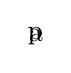
\begin{tikzpicture}[baseline=(base.base)]
  \node[inner sep=0pt] (base) at (0,0) {p};
  \node[inner sep=0pt] at (.02em,.04ex) {a};
\end{tikzpicture}%

\begin{tikzpicture}[baseline=(base.base)]
  \node[inner sep=0pt] (base) at (0,0) {a};
  \node[inner sep=0pt] at (.02em,-.02ex) {p};
\end{tikzpicture}%
le}'' au sens de Dynkin-Kostant. Alors le parabolique associé $P$ est un Borel (la réciproque n'étant pas vraie \deleted{sans doute}, cf table de Dynkin), et le groupe $Z_o$ est le groupe unité (i.e. $\operatorname{Dyn}_c$ est un torseur sous $G$),
% Serifed l contour plus an unresolved two-loop overprint; no order of impressions is assigned.
\unsure{
\begin{tikzpicture}[baseline=(base.base),x=1em,y=1ex]
  \node[anchor=base,inner sep=0pt] (base) at (0,0) {l};
  \draw[line width=.28pt] (.10,1.35) .. controls (-.30,1.62) and (-.29,.91) .. (-.03,.70)
    .. controls (.34,.52) and (.36,.18) .. (.13,.03)
    .. controls (-.10,-.02) and (-.31,.23) .. (-.18,.48);
  \draw[line width=.22pt] (-.08,-.28)--(-.08,.05);
  \draw[line width=.22pt] (.12,-.30)--(.12,.05);
  \draw[line width=.22pt] (.12,1.35)--(.30,1.29);
  \fill (.20,1.65) circle[radius=.025em];
\end{tikzpicture}}a réciproque n'étant pas vraie sans doute.
% slanted
\margin{\handwritten{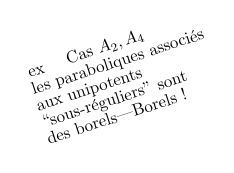
\begin{tikzpicture}[x=1em,y=1ex,scale=.61,transform shape]
  \begin{scope}[rotate=18]
    \node[anchor=base west,inner sep=0pt] at (0,0) {\uline{ex}};
    \node[anchor=base west,inner sep=0pt] at (2.4,.10) {Cas $A_2,A_4$};
    \node[anchor=base west,inner sep=0pt] at (-.10,-2.40) {les paraboliques associés};
    \node[anchor=base west,inner sep=0pt] at (-.15,-4.80) {aux unipotents};
    \node[anchor=base west,inner sep=0pt] at (-.15,-7.20) {``sous-réguliers'' sont};
    \node[anchor=base west,inner sep=0pt] at (-.15,-9.60) {des \unsure{borels|Borels} !};
  \end{scope}
\end{tikzpicture}}}
% archive sheet number: 19
